\documentclass{article}
\usepackage{settings}
%to write english paragraph \selectlanguage{language}
%to write english inline \textenglish{...}

\title{spring2018A}
\author{דורון שפיגל}
\date{02.04.24}

\begin{document}

\maketitle
\begin{Question}%1
בחומר מסוים נתונה הדיספרסיה של פס ההולכה:
\begin{equation*}
    \epsilon_{c}(k)= \epsilon_{0}+\frac{\hbar^2}{2}\left[ \left( \frac{k_{x}^4}{\alpha}-k_{x}^2 \right)\frac{1}{m_{1}}+\left( \frac{k_{y}^4}{\alpha}-k_{y}^2 \right)\frac{1}{m_{1}} + \frac{k_{z}^2}{m_{e}} \right]
\end{equation*}
נתון: $m_{1}=3m_{e}$, $\frac{\hbar^2\alpha}{2m_{1}}=1eV$ ו- $\epsilon_{0}=1eV$ והוא נמדד מהמקסימום של פס הערכיות הנמצא במרכז אזור ברילואין הראשון באנרגיה $\epsilon_{V}=0$.
\end{Question}
\begin{Answer}
תחילה אציב את הנתון $m_{1}=3m_{e}$ בנוסחה ואקבל:
\begin{align*}
        \epsilon_{c}(k)= \epsilon_{0}+\frac{\hbar^2}{2}\left[ \left( \frac{k_{x}^4}{\alpha}-k_{x}^2 \right)\frac{1}{3m_{e}}+\left( \frac{k_{y}^4}{\alpha}-k_{y}^2 \right)\frac{1}{3m_{e}} + \frac{k_{z}^2}{m_{e}} \right]\\
        \epsilon_{c}(k)= \epsilon_{0}+\frac{\hbar^2}{2m_{e}}\left[ \left( \frac{k_{x}^4}{\alpha}-k_{x}^2 \right)\frac{1}{3}+\left( \frac{k_{y}^4}{\alpha}-k_{y}^2 \right)\frac{1}{3} + k_{z}^2\right]
\end{align*}
נחשב את הגרדיאנט של הפונקציה ונמצא את הנקודות בהן היא מתאפסת:
\begin{align*}
    \nabla \epsilon_{c}(k)= \frac{\hbar^2}{2m_{e}}\left[ \left( \frac{4k_{x}^3}{\alpha}-2k_{x} \right)\frac{1}{3}+\left( \frac{4k_{y}^3}{\alpha}-2k_{y} \right)\frac{1}{3} + 2k_{z}\right]=0
\end{align*}
פתרון טריוויאלי הוא $k_{x}=k_{y}=k_{z}=0$. נבדוק את הנקודה הזו:
\begin{align*}
    \epsilon_{c}(0)= \epsilon_{0}+\frac{\hbar^2}{2m_{e}}\left[ 0+0+0\right]=\epsilon_{0}
\end{align*}
נחפש נקודות התאפסות על ידי השוואת מקדמים:
\begin{align*}
    \frac{4k_{x}^3}{\alpha}-2k_{x} = 0 \Rightarrow  k_{x}^2=\frac{\alpha}{2} &\Rightarrow k_{x}=\pm\sqrt{\frac{\alpha}{2}}\\
    \frac{4k_{y}^3}{\alpha}-2k_{y} = 0 \Rightarrow  k_{y}^2=\frac{\alpha}{2} &\Rightarrow k_{y}=\pm\sqrt{\frac{\alpha}{2}}\\
    2k_{z} = 0 &\Rightarrow k_{z}=0
\end{align*}
ולכן נקודות ההתאפסות של הגרדיאנט הן: ${\left\{ \vec{k}=\left( x,y,0 \right)\vert x,y = 0,\pm\sqrt{\frac{\alpha}{2}} \right\}}$.\\ עבור וקטורים מהצורות הבאות יש שיוויו מסימטריות משוואת הנפיצה בציר ה ${x,y}$. כך ש- 
\begin{align*}
    {\epsilon(\vec{k})=\epsilon((0,y,0))=\epsilon((x,0,0))}&= \epsilon_{0}+\frac{\hbar^2}{2m_{e}}\left[ \left( \frac{x^4}{\alpha}-x^2 \right)\frac{1}{3}\right]\\
    &=\epsilon_{0}+\frac{\hbar^2}{6m_{e}}\left[ \frac{\alpha}{2}^2\cdot\frac{1}{\alpha}-\frac{\alpha}{2} \right]\\
    &= - \frac{\hbar^{2} \alpha}{24 m_{e}} + \epsilon_{0} \underbrace{<}_{\frac{\hbar^2\alpha}{2m_1}=1>0}\epsilon_{0}\\
    \epsilon(\vec{k})=\epsilon((x,x,0))&=\epsilon_{0}+\frac{\hbar^2}{6m_{e}}\left[ \frac{\alpha}{2}^2\cdot\frac{1}{\alpha}-\frac{\alpha}{2} +\frac{\alpha}{2}^2\cdot\frac{1}{\alpha}-\frac{\alpha}{2} \right]\\
    &= - \frac{\hbar^{2} \alpha}{12 m_{e}} + \epsilon_{0} \underbrace{<}_{\frac{\hbar^2\alpha}{2m_1}=1>0}\epsilon_{0}
\end{align*}
כלומר:
\begin{equation*}
    \underbrace{\epsilon((x,x,0))}_{=- \frac{\hbar^{2} \alpha}{12 m_{e}} + \epsilon_{0}}<\underbrace{\epsilon((x,0,0))}_{=- \frac{\hbar^{2} \alpha}{24 m_{e}} + \epsilon_{0}}<\underbrace{\epsilon((0,0,0))}_{=\epsilon_{0}}
\end{equation*}
ולכן נקודות המינימום של פס ההולכה הן: $\vec{k}=\left( \pm\sqrt{\frac{\alpha}{2}},\pm\sqrt{\frac{\alpha}{2}},0 \right)$.\\
נתון כי $\epsilon_{0}=1eV,\quad \epsilon_{V}=0eV$.
\begin{align*}
    E_{gap}&=E_{Cmin}-E_{Vmax}=E_{Cmin}-0=E_{Cmin}\\
    &=  \frac{-\hbar^{2} \alpha}{12 m_{e}} + \epsilon_{0}=\frac{1}{2}\cdot \frac{-\hbar^{2} \alpha}{2 m_{1}}+\epsilon_{0}=\frac{-1}{2}eV+1eV=0.5eV
\end{align*}
נתון כי המקסימום של פס הערכיות נמצא במרכז אזור ברילואין הראשון באנרגיה $\epsilon_{V}=0$.כלומר:
$E_{Vmax}(\vec{k})=0\leftrightarrow \vec{k}=0$. לעומת זאת, ראינו ש $E_{Cmin}(\vec{k})\leftrightarrow \vec{k}\neq0$, לכן פער האנרגיה אינו ישר.\\ החומר אינו יכול לשמש עבור רכיבים פולטי אור מהסיבה שפוטונים מהווים מעברים כמעט אנכיים, ומכיוון שרק קצוות הפסים מאוכלסים, לא תוכל להתקיים פליטת פוטונים.\\
כעת נמצא את צפיפות המצבים \underline{בתחתית} פס ההולכה: כיוון שמדובר בתחתית הפס, נרצה לבצע קירוב פרבולי לפס האנרגיה בנקודות המינימום $\vec{k}=\left( \pm\sqrt{\frac{\alpha}{2}},\pm\sqrt{\frac{\alpha}{2}},0 \right)$. לפי משוואת הנפיצה הנתונה, ציר $\hat{z}$ פרבולי לחלוטין: $\left( \frac{\hbar^2}{2m_e}k_{z}^{2} \right)\hat{z}$, ואילו על צירי $\hat{x},\hat{y}$ נצטרך לבצע קירוב טיילור (מסדר שני).
\label{טור טיילור מסדר 2}
\begin{align*}
    \eval{f(x)}_{x=a}&\approx f(a)+f'(a)(x-a)+\frac{f''(a)}{2}(x-a)^2
    \tag{\textenglish{2nd order taylor for single variable}}\\
    \eval{f(x,y)}_{x=a,y=b}&\approx f(a,b)\\
    &+\eval{\od{f(x,y)}{x}}_{x=a,y=b}(x-a)+\eval{\od{f(x,y)}{y}}_{x=a,y=b}(y-b)\\
    &+\eval{\od[2]{f(x,y)}{x}}_{x=a,y=b}\frac{(x-a)^2}{2}+\eval{\od[2]{f(x,y)}{y}}_{x=a,y=b}\frac{(y-b)^2}{2}\\
    &+\eval{\od{}{y}\od{f(x,y)}{x}}_{x=a,y=b}(x-a)(y-b)
    \tag{\textenglish{2nd order taylor for two variables}}
    %(a,b)+fx(a,b)(x−a)+fy(a,b)(y−b)+fxx(a,b)2(x−a)2+fxy(a,b)(x−a)(y−b)+fyy(a,b)2(y−b)2
\end{align*}
אחשב כל גורם של הסכום עבור $f(x,y)=\epsilon_{c}(k_{min})$:
\begin{align*}
    \epsilon_{c}\left(k(x,y,0)\right)&= \epsilon_{0}+\frac{\hbar^2}{2m_{e}}\left[ \left( \frac{k_{x}^4}{\alpha}-k_{x}^2 \right)\frac{1}{3}+\left( \frac{k_{y}^4}{\alpha}-k_{y}^2 \right)\frac{1}{3} + k_{z}^2\right]\\
    &= \epsilon_{0}-\frac{\hbar^2\alpha}{12m_e}=0.5eV=E_{gap}\\
    \eval{\od{\epsilon_{c}\left(k(x,y,0)\right)}{k_{x}}}_{\begin{matrix}
        a=k_{xmin}\\
        b=k_{ymin}
    \end{matrix}}\left( k_{x}-k_{xmin} \right)&= 
    \frac{\hbar^2}{2m_{e}}\left[ \left( \frac{4k_{xmin}^3}{\alpha}-2k_{xmin} \right)\frac{1}{3}\right]\left( k_{x}-k_{xmin} \right)=0\\
    \eval{\od{\epsilon_{c}\left(k(x,y,0)\right)}{k_{y}}}_{\begin{matrix}
        a=k_{xmin}\\
        b=k_{ymin}
    \end{matrix}}\left( k_{y}-k_{ymin} \right)&=0\\
    \eval{\od[2]{\epsilon_{c}\left(k(x,y,0)\right)}{k_{x}}}_{\begin{matrix}
        a=k_{xmin}\\
        b=k_{ymin}
    \end{matrix}}\frac{(k_{x}-k_{xmin})^2}{2}&=\frac{\hbar^2}{2m_{e}}\left[ \left( \frac{12k_{xmin}^2}{\alpha}-2\right)\frac{1}{3}\right]\frac{(k_{x}-k_{xmin})^2}{2}\\
    &=\frac{\hbar^{2}}{12m_{e}} \left( \frac{12k_{xmin}^2}{\alpha}-2\right)\left( k_{x}-k_{xmin} \right)^{2}\\
    \left[ k_{xmin}=\sqrt{\frac{\alpha}{2}} \right]\Rightarrow &=\frac{\hbar^{2}}{12m_{e}} \left( \frac{12\cdot\frac{\alpha}{2}}{\alpha}-2\right)\left( k_{x}-\sqrt{\frac{\alpha}{2}} \right)^{2}\\
    &=\frac{\hbar^{2}}{3m_{e}}\left( k_{x}-\sqrt{\frac{\alpha}{2}} \right)^{2}\\
    \eval{\od[2]{\epsilon_{c}\left(k(x,y,0)\right)}{k_{y}}}_{\begin{matrix}
        a=k_{xmin}\\
        b=k_{ymin}
    \end{matrix}}\frac{(k_{y}-k_{ymin})^2}{2}&=\frac{\hbar^{2}}{3m_{e}}\left( k_{y}-\sqrt{\frac{\alpha}{2}} \right)^{2}
\end{align*}
עבור כל הצירים נקבל בסך הכל:
\begin{align*}
    \eval{\epsilon_{c}\left( k(x,y,z) \right)}_{kmin}=E_{gap}+\frac{\hbar^{2}}{3m_{e}}\left( \left( k_{x}-\sqrt{\frac{\alpha}{2}} \right)^{2}+\left( k_{y}-\sqrt{\frac{\alpha}{2}} \right)^{2} \right)+\frac{\hbar^{2}}{2m_{e}}k_{z}^{2}
\end{align*}
יחס הנפיצה הוא פרבולי (עד כדי הזזה הזזות בצירים $\hat{x},\hat{y}$), אולם, המסות האפקטיביות בצירים $\hat{x},\hat{y}$ שונות מהמסה האפקטיבית בציר $\hat{z}$, כדי לקבל צפיפות מצבים, נשתמש בקירוב של צפיפות המצבים להולכה:\\
\underline{שלב 1:} חישוב המסה האפקטיבית לכל ציר:
\begin{align*}
    m^{*}=\boxed{\left( \frac{1}{\hbar^{2}} \od[2]{E}{k} \right)^{-1}}\\
    m_{x}^{*}&=\left( \frac{1}{\hbar^{2}} \od[2]{E}{k_{x}} \right)^{-1}=\left( \frac{1}{\hbar^{2}} \frac{2\hbar^{2}}{3m_{e}} \right)^{-1}=\frac{3m_{e}}{2}=1.5m_{e}\\
    m_{y}^{*}&=1.5m_{e}\\
    m_{z}^{*}&=\left( \frac{1}{\hbar^{2}} \od[2]{E}{k_{z}} \right)^{-1}=\left( \frac{1}{\hbar^{2}} \frac{2\hbar^{2}}{2m_{e}} \right)^{-1}=m_{e}
\end{align*}
\underline{שלב 2:} הצגת טנזור המסה האפקטיבית:
\begin{equation*}
    \frac{1}{m^{*}}=\begin{pmatrix}
        \frac{1}{m_{x}^{*}} & 0 & 0\\
        0 & \frac{1}{m_{y}^{*}} & 0\\
        0 & 0 & \frac{1}{m_{z}^{*}}
    \end{pmatrix}= \begin{pmatrix}
        \frac{1}{1.5m_{e}} & 0 & 0\\
        0 & \frac{1}{1.5m_{e}} & 0\\
        0 & 0 & \frac{1}{m_{e}}
    \end{pmatrix}
\end{equation*}
\underline{שלב 3:} חישוב הסקלר $m^{*}$:
\begin{align*}
    \det{\frac{1}{m^{*}}}&=\begin{vmatrix}
        \frac{1}{1.5m_{e}} & 0 & 0\\
        0 & \frac{1}{1.5m_{e}} & 0\\
        0 & 0 & \frac{1}{m_{e}}
    \end{vmatrix} = \frac{4}{9 m_{e}^{3}}\\
    m^{*}&=\frac{9 m_{e}^{3}}{4}=2.25m_{e}^{3}
\end{align*}
\underline{שלב 4:} המסה האפקטיבית של צפיפות המצבים:\\
לפי התרגול, המסה האפקטיבית של צפיפות המצבים היא:
\begin{equation}\label{המסה האפקטיבית של צפיפות מצבים}
    g(E)=\frac{m_{DOS}^{\frac{3}{2}}\sqrt{2}}{\pi^{2}\hbar^{3}}\sqrt{E-E_{C}},\quad m_{DOS}=g_{V}^{\frac{2}{3}}\left( m_{1}m_{2}m_{3} \right)^{\frac{1}{3}}
\end{equation}
כאשר $m_{1},m_{2},m_{3}$ המסות האפקטיביות לאורך 3 הצירים הראשיים של הבעיה.\\
$g_{V}$ - פרמטר הניוון המעיד על מספר המשטחים שווי האנרגיה בתוך אזור ברילואן הראשון.\\
במקרה של תרגיל זה, ראינו כי יש 4 מינימות $\vec{k}=\left( \pm\sqrt{\frac{\alpha}{2}},\pm\sqrt{\frac{\alpha}{2}},0 \right)$, ולכן פרמטר הניוון הוא $g_{V}=4$, ונקבל:
$$m_{DOS}=4^{\frac{2}{3}}\left( m_{1}m_{2}m_{3} \right)^{\frac{1}{3}}=4^{\frac{2}{3}}\left( m^{*} \right)^{\frac{1}{3}}\approx3.301m_{e}$$
\underline{שלב 5:} צפיפות נושאי מטען:\\
מקורס מל"מ, ידוע כי צפיפות נושאי המטען נתונה על ידי:
\begin{equation}\label{צפיפות נושאי מטען}
    \underbrace{n}_{\text{צפיפות נושאי מטען}}=\int_{-\infty}^{\infty}\underbrace{g(E)}_{\text{צפיפות מצבים}}\,\cdot\underbrace{f_{FD}{(E)}}_{\text{אכלוס פרמי דיראק}}dE
\end{equation}
נניח שהחומר נמצא בטמפרטורה של $T=0[K]$, לכן התפלגות הפרמי דיראק תתנהג כמדרגה: $f_{FD}{(E)}=\begin{cases}
    1 & E\leq \mu_c=E_{f}\\
    0 & E>\mu_c=E_{f}
\end{cases}$. נבחר את אנרגיית הייחוס $E_c=0$ ומתקיים:
\begin{align*}
    n&=\int_{-\infty}^{\infty}g(E)\cdot f_{FD}dE=\int_{E_{c}}^{E_{f}}
    \frac{m_{DOS}^{\frac{3}{2}}\sqrt{2}}{\pi^{2}\hbar^{3}}\sqrt{E-E_{C}}f_{FD}{(E)}dE\\
    &=\int_{0}^{E_{f}}\frac{m_{DOS}^{\frac{3}{2}}\sqrt{2}}{\pi^{2}\hbar^{3}}\sqrt{E}dE
    =\frac{m_{DOS}^{\frac{3}{2}}\sqrt{2}}{\pi^{2}\hbar^{3}}\int_{0}^{E_{f}}\sqrt{E}dE\\
    &=\frac{m_{DOS}^{\frac{3}{2}}\sqrt{2}}{\pi^{2}\hbar^{3}}\left[ \frac{2}{3}E^{\frac{3}{2}} \right]_{0}^{E_{f}}=\frac{2}{3}\frac{m_{DOS}^{\frac{3}{2}}\sqrt{2}}{\pi^{2}\hbar^{3}}E_{f}^{\frac{3}{2}}
\end{align*}
בשאלה זאת נתון לנו ש $n=10^{18}cm^{-3} = 10^{24}m^{-3}$, ושואלים מהו ערכו של רמת הפרמי. נציב את $n$ ונפתור את המשוואה:
\begin{align*}
    E_{f}&=\left( \frac{3\pi^{2}\hbar^{3}n}{2m_{DOS}^{\frac{3}{2}}\sqrt{2}} \right)^{\frac{2}{3}}\\
    &=\left( \frac{3\cdot \pi^{2}}{2\sqrt{2}} \right)^{\frac{2}{3}}\frac{\hbar^2}{m_{DOS}}n^{\frac{2}{3}}\\
    &=4.78\cdot10^{16}\cdot \frac{\hbar^2}{m_{DOS}}\\
    \begin{cases}
        \hbar=1.054\cdot 10^{-34}Js\\
        m_{DOS}=3.301m_{e}=3.301\cdot 9.11\cdot 10^{-31}kg
    \end{cases}\rightarrow &=4.78\cdot10^{16}\cdot0.037\cdot10^{-37}\\
    &\boxed{E_{f}=1.7686 \cdot 10^{-22}[J]}
\end{align*}
\end{Answer}
\begin{Question}%2
נתונה שרשרת חד ממידית של אטומים בעלי מסה $m$ במרחק $d$ זה מזה. קבוע הכוח (הקפיץ) בין שני אטומים סמוכים משתנה לסירוגין בין הערכים ${\alpha,\,\beta}$.
\end{Question}
\begin{Answer}
קיומם של שני קבועי קפיץ שונים משמעו שישנו תא יחידה כשלהוא כיוון שאנו מחפשים סימטריה כלשהי בשרשרת. נבחר תא יחידה כזה שמקיים סימטריות בשרשרת:\\ 
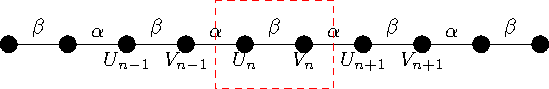
\includegraphics[width=\textwidth]{image/Q2image.pdf}
פוטנציאל האנרגיה של התא, הוא:
\begin{itemize}
    \item הפוטנציאל בין שני האטומים: $U=\frac{1}{2}\underbrace{\beta}_{\text{קפיץ}}\underbrace{(v_{n}-u_{n})^{2}}_{\text{המרחק}}$.
    \item הפוטנציאל בין האטום השמאלי לקבוע הקפיץ: $U=\frac{1}{2}\alpha(u_{n}-v_{n-1})^{2}$.
    \item הפוטנציאל בין האטום הימני לקבוע הקפיץ: $U=\frac{1}{2}\alpha(u_{n+1}-v_{n})^{2}$.
\end{itemize}
כלומר, פוטנציאל האנרגיה של התא הוא:
\begin{equation*}
    U=\frac{1}{2}\alpha(u_{n+1}-v_{n})^{2}+\frac{1}{2}\beta(v_{n}-u_{n})^{2}+\frac{1}{2}\alpha(u_{n}-v_{n-1})^{2}
\end{equation*}
לכל אטום, נרשום את משוואת הכוח (שהיא נגזרת מהפוטנציאל $F=-\od{U}{x}$):
\begin{align*}
    \begin{cases}
        u_{n}:\underbrace{-}_{\leftarrow}\alpha\left( u_{n}-v_{n-1} \right)\underbrace{+}_{\rightarrow}\beta\left( v_{n}-u_{n} \right)\\
        v_{n}:\underbrace{-}_{\leftarrow}\beta\left( v_{n}-u_{n} \right)\underbrace{+}_{\rightarrow}\alpha\left( u_{n+1}-v_{n} \right)
    \end{cases}
\end{align*}
נגדיר גל מישורי:
\begin{align*}
    \begin{cases}
        u_{n}=Ae^{iknd - i\omega t}\\
        v_{n}=Be^{iknd -ikd - i\omega t}
    \end{cases}
\end{align*}
נציב למשוואות הכוח ונקבל:
\begin{align*}
    &\left\{\begin{aligned}
        &-m\omega^{2}Ae^{iknd - i\omega t}&=-\alpha\left( Ae^{iknd - i\omega t}-Be^{ik(n-1)d -ikd - i\omega t} \right)\\&&+\beta\left( Be^{iknd -ikd - i\omega t}-Ae^{iknd - i\omega t} \right)\\
        &-m\omega^{2}Be^{iknd -ikd - i\omega t} &= -\beta\left( Be^{iknd -ikd - i\omega t}-Ae^{iknd - i\omega t} \right)\\&&+\alpha\left( Ae^{ik(n+1)d - i\omega t}-Be^{iknd -ikd - i\omega t} \right)
    \end{aligned}\right.\\
    \xrightarrow[\div e^{iknd - i\omega t}]{\div e^{iknd - i\omega t}}&
    \begin{cases}
        -m\omega^{2}A=-\alpha\left( A-Be^{-2ikd} \right)+\beta\left( Be^{-ikd}-A \right)\\
        -m\omega^{2}Be^{-ikd} = -\beta\left( Be^{-ikd}-A \right)+\alpha\left( Ae^{ikd}-Be^{-ikd} \right)
    \end{cases}\\
    \xrightarrow[\div e^{-kd}]{}&
    \begin{cases}
        -m\omega^{2}A=-\alpha\left( A-Be^{-2ikd} \right)+\beta\left( Be^{-ikd}-A \right)\\
        -m\omega^{2}B = -\beta\left( B-Ae^{ikd} \right)+\alpha\left( Ae^{2ikd}-B \right)
    \end{cases}\\
    \rightarrow&
    \begin{cases}
        A\left( \alpha+\beta-m\omega^2 \right)+B\left( -\alpha e^{-2ikd}-\beta e^{-ikd} \right)=0\\
        A\left( -\alpha e^{2ikd}-\beta e^{ikd} \right)+B\left( \alpha+\beta-m\omega^2 \right)=0
    \end{cases}
\end{align*}
נקבל את המטריצה האופיינית, ונשווה את הדטרמיננטה שלה לאפס:
\begin{align*}
    &\begin{pmatrix}
        \alpha+\beta-m\omega^2&-\alpha e^{-2ikd}-\beta e^{-ikd}\\
        -\alpha e^{2ikd}-\beta e^{ikd}&\alpha+\beta-m\omega^2 
    \end{pmatrix}
    \begin{pmatrix}
        A\\
        B
    \end{pmatrix}=
    \begin{pmatrix}
        0\\
        0
    \end{pmatrix}\\
    &\begin{vmatrix}
        \alpha+\beta-m\omega^2&-\alpha e^{-2ikd}-\beta e^{-ikd}\\
        -\alpha e^{2ikd}-\beta e^{ikd}&\alpha+\beta-m\omega^2 
    \end{vmatrix}\\
    &=\left( \alpha+\beta-m\omega^2 \right)^{2}-\left( -\alpha e^{-2ikd}-\beta e^{-ikd} \right)\left( -\alpha e^{2ikd}-\beta e^{ikd} \right)\\
    &= \left( \alpha+\beta-m\omega^2 \right)^{2} - \left( \alpha^2+\alpha\beta e^{-ikd} +\alpha\beta e^{ikd} +\beta^2\right)
\end{align*}
ניזכר בזהות אויילר לקוסינוס:
$$\cos(X)=\frac{e^{iX}+e^{-iX}}{2}$$
כך ש:
\begin{align*}
    \left( \alpha^2+\alpha\beta e^{-ikd} +\alpha\beta e^{ikd} +\beta^2\right)=\alpha^{2}+\beta^{2}+2\alpha\beta\cos(kd)
\end{align*}
ובפירוק של הגורם השמאלי:
\begin{align*}
    \left( \alpha+\beta-m\omega^2 \right)^{2}&= \left( \left[ \alpha+\beta \right]-m\omega^2 \right)^{2}=\left[ \alpha+\beta \right]^{2}-2\left[ \alpha+\beta \right]m\omega^2+m^{2}\omega^{4}\\
    &=\alpha^{2}+\beta^{2}+2\alpha\beta-2\left[ \alpha+\beta \right]m\omega^2+m^{2}\omega^{4}
\end{align*}
ולכן, במשוואת הדטרמיננטה:
\begin{align*}
    &\left( \alpha+\beta-m\omega^2 \right)^{2} - \left( \alpha^2+\alpha\beta e^{-ikd} +\alpha\beta e^{ikd} +\beta^2\right)\\
    &=2\alpha\beta+2\alpha\beta\cos(kd)-2\left[ \alpha+\beta \right]m\omega^2+m^{2}\omega^{4}\\
    &=2\alpha\beta\left( 1+\cos(kd) \right)-2\left[ \alpha+\beta \right]m\omega^2+m^{2}\omega^{4}\\
    &=4\alpha\beta\left( \frac{1+\cos(kd)}{2} \right)-2\left[ \alpha+\beta \right]m\omega^2+m^{2}\omega^{4}
\end{align*}
ניזכר בזהות $\sin^{2}X=\frac{1-\cos2X}{2}$ כך ש:
\begin{align*}
    &4\alpha\beta\left( \frac{1+\cos(kd)}{2} \right)-2\left[ \alpha+\beta \right]m\omega^2+m^{2}\omega^{4}\\&=4\alpha\beta\sin^{2}\left( \frac{kd}{2} \right)-2\left[ \alpha+\beta \right]m\omega^2+m^{2}\omega^{4}\\
    \xrightarrow{\div m^{2}}&=\omega^{4}-\frac{2\left[ \alpha+\beta \right]}{m}\omega^{2}+\frac{4\alpha\beta}{m^2}\sin^{2}\left( \frac{kd}{2} \right)=0\\
    \xrightarrow{\omega^{2}=w}&w^{2}-\frac{2\left[ \alpha+\beta \right]}{m}w+\frac{4\alpha\beta}{m^2}\sin^{2}\left( \frac{kd}{2} \right)=0\\
    w_{1,2}&=\frac{\alpha+\beta}{m} \pm \frac{1}{2}\sqrt{\frac{4}{m^2}\left[ \alpha+\beta \right]^{2}-\frac{16\alpha\beta}{m^2}\sin^{2}\left( \frac{kd}{2} \right)}\\
    w_{1,2}&=\frac{\alpha+\beta}{m} \pm \frac{1}{2}\sqrt{\frac{4}{m^2}\left(\left[ \alpha+\beta \right]^{2}-4\alpha\beta\sin^{2}\left( \frac{kd}{2} \right) \right)}\\
    w_{1,2}&=\frac{\alpha+\beta}{m} \pm \frac{1}{m}\sqrt{\left[ \alpha+\beta \right]^{2}-4\alpha\beta\sin^{2}\left( \frac{kd}{2} \right) }\\
    \xRightarrow{\omega=\abs{\sqrt{w^{2}}}}&\omega_{1,2}=\abs{\sqrt{\frac{\alpha+\beta}{m} \pm \frac{1}{m}\sqrt{\left[ \alpha+\beta \right]^{2}-4\alpha\beta\sin^{2}\left( \frac{kd}{2} \right) }}}
\end{align*}
כיוון שהשורש מחזיר מספר חיובי, נקבל שעבור סימן $+$ נקבל תדר גדול יותר, כלומר אופן של גלים אופטיים. עבור סימן $-$ נקבל תדר קטן יותר, כלומר אופן של גלים אקוסטיים.\\
נתון כעת כי $k=0$, נמצא את הערכים העצמיים והווקטורים העצמיים:
\begin{align*}
    \omega_{1,2}\left( k=0 \right)&=\abs{\sqrt{\frac{\alpha+\beta}{m} \pm \frac{1}{m}\sqrt{\left[ \alpha+\beta \right]^{2} }}}=\abs{\sqrt{\frac{\alpha+\beta}{m} \pm \frac{\alpha+\beta}{m} }}\\
    &\Rightarrow\begin{cases}
        \omega_1=0&\text{אופן של גלים אקוסטיים}\\
        \omega_2=\sqrt{\frac{2\left( \alpha+\beta \right)}{m}}&\text{אופן של גלים אופטיים}
    \end{cases}
\end{align*}
נציב את $\omega_1=0,\quad k=0$ במטריצה ונמצא את הווקטור העצמי:
\begin{align*}
    &\begin{pmatrix}
        \alpha+\beta-m\omega^2&-\alpha e^{-2ikd}-\beta e^{-ikd}\\
        -\alpha e^{2ikd}-\beta e^{ikd}&\alpha+\beta-m\omega^2 
    \end{pmatrix}
    \begin{pmatrix}
        A\\
        B
    \end{pmatrix}=
    \begin{pmatrix}
        0\\
        0
    \end{pmatrix}\\
    &\begin{pmatrix}
        \alpha+\beta&-\alpha -\beta\\
        -\alpha -\beta &\alpha+\beta
    \end{pmatrix}
    \begin{pmatrix}
        A\\
        B
    \end{pmatrix}=
    \begin{pmatrix}
        0\\
        0
    \end{pmatrix}\rightarrow A=B\rightarrow\begin{bmatrix}1\\1\end{bmatrix}\rightarrow\frac{1}{\sqrt{2}}\begin{pmatrix}
        1\\1
    \end{pmatrix}
\end{align*}שתי האמפליטודות זהות סימנן, כלומר כל תא היחידה נע ביחד, דבר המצופה למוד האקוסטי.\\
נציב $\omega_2=\sqrt{\frac{2\left( \alpha+\beta \right)}{m}}$ במטריצה ונמצא את הווקטור העצמי:
\begin{align*}
    &\begin{pmatrix}
        \alpha+\beta-m\omega^2&-\alpha e^{-2ikd}-\beta e^{-ikd}\\
        -\alpha e^{2ikd}-\beta e^{ikd}&\alpha+\beta-m\omega^2 
    \end{pmatrix}
    \begin{pmatrix}
        A\\
        B
    \end{pmatrix}=
    \begin{pmatrix}
        0\\
        0
    \end{pmatrix}\\
    &\begin{pmatrix}
        -\alpha-\beta&-\alpha -\beta\\
        -\alpha -\beta &-\alpha-\beta
    \end{pmatrix}
    \begin{pmatrix}
        A\\
        B
    \end{pmatrix}=
    \begin{pmatrix}
        0\\
        0
    \end{pmatrix}\rightarrow A=-B\rightarrow\begin{bmatrix}-1\\1\end{bmatrix}\rightarrow\frac{1}{\sqrt{2}}\begin{pmatrix}
        -1\\1
    \end{pmatrix}
\end{align*}
שתי האמפליטודות הפוכות בסימנן, דבר המצופה למוד האופטי, הרכיבים של תא היחידה יהיו בעלי כיווני תנועה מנוגדים.
\end{Answer}


\begin{Question}%3
נתונה מערכת בת שלוש רמות, הרמה הראשונה בעלת אנרגיה 0, הרמה השנייה בעלת אנרגיה $\epsilon$ והרמה השלישית בעלת אנרגיה $50\epsilon$.
\end{Question}
\begin{Answer}
הנוסחה לחישוב פונקציית החלוקה $Z$ היא:
\begin{align}\label{פונקציית החלוקה}
    1&=\sum \limits^{}_{S}{P\left( s \right)}=\frac{1}{Z}\sum \limits^{}_{S}{e^{-\beta E\left( s \right)}}\\
    \rightarrow&Z\triangleq \sum \limits^{}_{S}{e^{\frac{-E\left( s \right)}{kT} }}=\sum \limits^{}_{S}{e^{-\beta E\left( s \right)}}
\end{align}
נציב את הערכי האנרגיה של הרמות ונקבל:
\begin{equation*}
    Z\triangleq \sum \limits^{}_{n}{e^{-\beta E_{n}}}=e^{-\beta\cdot0}+e^{-\beta\epsilon}+e^{-\beta 50\epsilon}=1+e^{-\beta\epsilon}+e^{-\beta 50\epsilon}
\end{equation*}
הנוסחה לחישוב האנרגיה הממוצעת על ידי פונקציית החלוקה היא:
\begin{align}\label{אנרגיה ממוצעת}
    \begin{cases}
        \langle E \rangle=\sum \limits^{}_{S}{E\left( s \right)P\left( s \right)}=\frac{1}{Z}\sum \limits^{}_{S}{E\left( s \right)e^{-\beta E\left( s \right)}}\\
        \pd{Z}{\beta}=\pd{}{\beta}\sum \limits^{}_{S}{e^{-\beta E\left( s \right)}}=-\sum \limits^{}_{S}{E\left( s \right)e^{-\beta E\left( s \right)}}
    \end{cases}\\
    \langle E \rangle=-\frac{1}{Z}\pd{Z}{\beta}\leftrightarrow\langle E \rangle=-\pd{}{\beta}\ln{Z}
\end{align}
נציב את ערכי האנרגיה של הרמות ופונקציית החלוקה בנוסחה ונקבל:
\begin{align*}
    \langle E \rangle&=\frac{1}{Z}\sum \limits^{}_{n}{E_{n}e^{-\beta E_{n}}}\\
    &=\frac{1}{Z}\left[ 0\cdot e^{-\beta\cdot0} +\epsilon\cdot e^{-\beta\epsilon}+50\epsilon\cdot e^{-\beta 50\epsilon}\right]\\
    &=\frac{\epsilon\cdot e^{-\beta\epsilon}+50\epsilon\cdot e^{-\beta 50\epsilon}}{1+e^{-\beta\epsilon}+e^{-\beta 50\epsilon}}
\end{align*}
הגרפים המתקבלים הם:\\
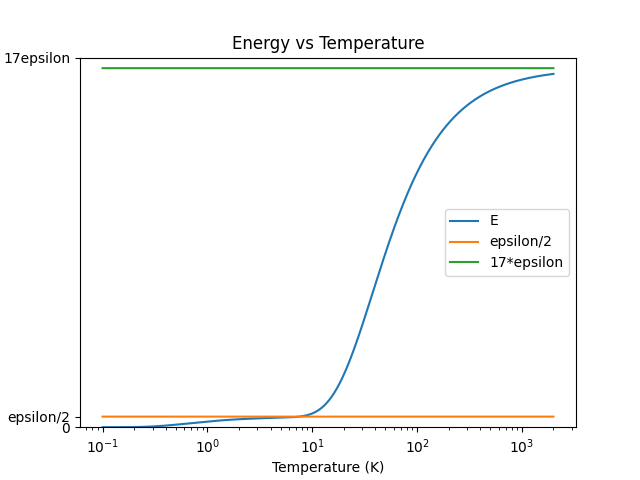
\includegraphics[width=0.9\textwidth]{image/Q3energy.png}\\
בטמפרטורה נמוכה מאוד, קרוב לאפס, רק הרמה הבסיסית מאוכלסת, כאן נתון שהרמת הזאת היא אנרגיה 0, אז שם הגרף מתחיל. חשוב לציין שזה קורה עבור \textbf{הרמה הנמוכה ביותר} כלומר, אם בתרגיל הרמה הכי נמוכה הייתה ערך אחר שלא אפס אז הגרף היה מתחיל מערך הזה ולא אפס.\\
עם גדילת הטמפרטורה, נוסף חום למערכת ואלקטרונים מתחילים לעבור בין הרמה הבסיסית לרמה האמצעית, זאת העלייה הראשונה בגרף, כאשר מגיעים לטמפרטורה מסוימת יש מספיק חום כך שההסתברות של חלקיק להיות ברמה 0 או רמה 1 שווה ולכן ממוצע האנרגיה הוא סכום 2 הרמות חלקי מספר הרמות: $\frac{0+\epsilon}{2}=\frac{\epsilon}{2}$.\\
בין רמה 2 לרמה 3 שוב קורה תהליך דומה ואז ממוצע האנרגיה הוא $\frac{0+\epsilon+50\epsilon}{2}=\frac{51\epsilon}{3} = 17 \epsilon$.\\
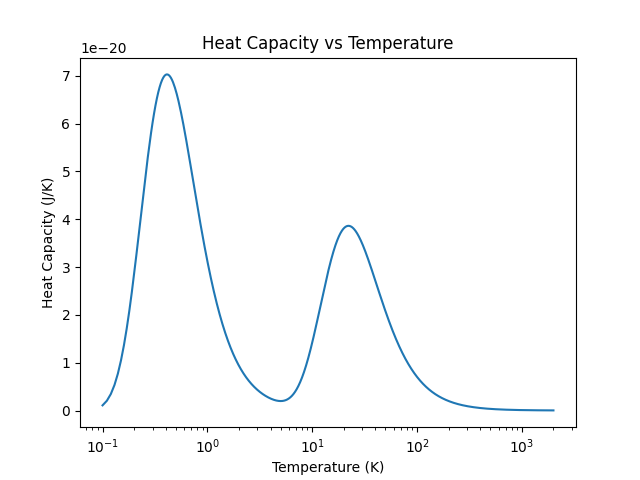
\includegraphics[width=0.9\textwidth]{image/Q3HeatCapacity.png}\\
גרף הקיבול חום הוא למעשה נגזרת גרף הממוצע אנרגיה.\\
בטמפרטורה נמוכה מאוד, קרוב לאפס, לפי החוק השלישי של התרמודינמיקה, קיבול החום שואף לאפס בטמפרטורות השואפות לאפס.\\
כאשר אנרגיית המערכת $E_{Therm}\sim \epsilon$ מתאפשר מעבר בין 2 הרמות התחתונות וקיבול החום מקבל ערך שאינו אפס. - עד השיא הראשון בגרף.\\
עבור אנרגיית מערכת $\epsilon<<E_{Therm}<<50\epsilon$ שתי הרמות התחתונות מאוכלסות בצורה שווה ולכן האנרגיה הממוצעת מתקבעת על הערך הממוצע של שתיהן בלבד (הפס הכתום בגרף האנרגיה הממוצעת), מכיוון ששתי הרמות האלה מאוכלסות בצורה שווה, קיבול החום שוב דועך לאפס כי לא ניתן לעבור בין המצבים.\\
עבור $E_{Therm}\sim 50\epsilon$ מתאפשר מבער בין הרמה השנייה לשלישית, ורואים את השיא השני בגרף קיבול החום.\\
עבור $E_{Therm}>> 50\epsilon$ כל הרמות מאוכלסות בצורה שווה וקיבול החום שואף לאפס.
\end{Answer}

\begin{Question}%4
ענו על הסעיפים הבאים בקצרה.\\
\begin{SubQuestion}
עבור מחסום פוטנציאל ריבועי, הסבירו: מדוע ישנן אנרגיות אשר בהן מתקבל שיא בהסתברות למנהור?
\end{SubQuestion}
\begin{SubAnswer}
עבור אנרגיות הגבוהות מערכו של המחסום, מתקבלים שיאים בהסתברות למנהור החלקיק. הסיבה לכך היא שאורך הגל של החלקיק תואם לרוחב המחסום ואנו מקבלים מצב רזונטיבי. תופעה זו מתקיימת באופן הרבה יותר חזק עבור 2 מחסומים בעלי מרווח כלשהו ביניהם.
\end{SubAnswer}
\begin{SubQuestion}
הצדיקו את השימוש בקירוב יחס הנפיצה הפרבולי עבור צפיפות המצבים במוליכים למחצה.
\end{SubQuestion}
\begin{SubAnswer}
עבור מוליכים למחצה, רמת פרמי נמצאת בתוך הפס האסור במיקום כלשהו. הן פס ההולכה והן פס הערכיות רואים רק את הזנבות של ההתפלגות, כלומר שרק קצוות הפסים הקרובים לפער האסור יכילו חלקיקים. זכרו שהרוחב הטיפוסי של כל פס הוא כאלקטרון - וולט אולם התפלגות פרמי - דיראק משתנה על סקאלה של מיליאלקטרון - וולטים, או כמה עשרות שלהם לכל היותר, ולכן מסתכלים רק על קצוות הפסים בהם הקירוב הפרבולי תופס.
\end{SubAnswer}
\begin{SubQuestion}
בדרך כלל המסה האפקטיבית של אלקטרון במתכת גדולה יותר ממסתו בוואקום $(m_{e})$. הסבירו מדוע.
\end{SubQuestion}
\begin{SubAnswer}
מתכות הן חומרים אשר בהן רמת פרמי נמצאת יחסית עמוק בתוך אחד מהפסים המותרים. ראינו שבעומק הפסים מסת האלקטרון שואפת לאינסוף (או מינוס אינסוף) ולכן נצפה למסה אפקטיבית גדולה הרבה יותר ממסת האלקטרון בוואקום.
\end{SubAnswer}
\begin{SubQuestion}
    מה המשמעות הפיזיקלית של קירוב התפלגויות בוזה - איינשטיין ופרמי - דיראק להתפלגות מקסוול - בולצמן מבחינת האופי של החלקיקים?
\end{SubQuestion}
\begin{SubAnswer}
    הן התפלגויות בוזה - איינשטיין והתפלגות פרמי - דיראק הן התפלגויות המאפיינות חלקיקים קוונטים ואשר נובעות מהיותם בוזונים או פרמיונים. אשר אנו מבצעים קירוב להתפלגות מקסוול - בולצמן הקלאסית, אנו מזניחים את האופי הקוונטי של החלקיקים בבעיה והופכים אותם לחלקיקים קלאסים - יש מעט חלקיקים והמון מצבי אנרגיה פנויים כך שהחלקיקים אינם זה בזה ואופיים הקוונטי אינו בא לידי ביטוי.
\end{SubAnswer}
\begin{SubQuestion}
    ראינו שעבור שריג כלשהוא, ניתן לתאר פונונים ואלקטרונים על ידי דיאגרמות פסי אנרגיה. בכל זאת ישנם מספר הבדלים בין הדיאגרמות של שני החלקיקים. ציינו מהם והסבירו את מקורם הפיזיקלי.
\end{SubQuestion}
\begin{SubAnswer}
\begin{enumerate}
    \item דיאגרמות הפסים של האלקטרונים מכילות מספר אינסופי של פסים בעוד שמספר הפסים עבור פונונים מוגבל אינהרנטית (כתלות במורכבות תא היחידה). הדבר נובע מהפוטנציאל של כל אטום אשר מהווה בור פוטנציאל אינסופי הגורר אינסוף מצבי אנרגיה.
    \item סקאלות האנרגיה של שתי הדיאגרמות שונות משמעותית. עבור אלקטרונים מדובר באלקטרון - וולטים בעוד שעבור פונונים מדובר במילי - אלקטרון - וולטים. המקור הפיזיקלי במקרה זה הוא הכוח אותו מפעילים האטומים זה על זה (מה שמניב את קבוע הקפיץ), לעומת רמות האנרגיה הטיפוסיות של האטום שהן בסקאלות של אלקטרון - וולטים.
    \item הפסים האלקטרונים נובעים ממצבים אטומיים ממוקמים (אורביטלים) בעוד שהפונונים מבוססים על תנודות בכול הגביש, שאינן נובעות רק מתא היחידה הבודד.
    \item יחס הנפיצה תמיד מכיל מקטע לינארי סביב $k=0$ (היכן שאנו מחשבים את מהירות הקול).
\end{enumerate}
\textcolor{red}{\textbf{לא נכון:} פונונים הם בוזונים לעומת אלקטרונים שהם פרמיונים. מבני הפסים השונים לא מבוסס על היות של החלקיקים פרמיונים/ בוזונים!}
\end{SubAnswer}
\begin{SubQuestion}
במוליכים למחצה, לרוב מוסיפים מסממים מסוגים שונים על מנת להגדיל את כמות נושאי המטען (אלקטרונים או חורים). האטומים המסממים הם לרוב בריכוז של כ- ${10^{14} - 10^{17}\left[ cm^{-3} \right]}$. מדוע על אף נוכחות האטומים הזרים (שסידורים יכול להיות רנדומלי לחלוטין) אנו עדיין מתייחסים לשריג כאל מבנה מחזורי מסודר?
\end{SubQuestion}
\begin{SubAnswer}
מספר האטומים הטיפוסי בחומר מאקרוסקופי הוא בערך מספר אבוגדרו. מספר זה גדול בכמה סדרי גודל מרמת המסממים שאנו מחדירים בדרך כלל ולכן בקירוב טוב מאוד ניתן להתעלם מהשפעת המסממים על מבנה השריג.\\
הערה: אם מגדילים את כמות המסממים, בשלב מסוים האטומים המסממים יתחילו להרגיש זה את זה וליצור פס אנרגיה חדש משלהם (לתופעה זו קוראים גם היווצרות פער אנרגיה והיא מתרחשת עבור סימום כבד של השריג).
\end{SubAnswer}
\begin{SubQuestion}
הצדיקו את המשפט: פסי אנרגיה מלאים אינם תורמים להולכה חשמלית.
\end{SubQuestion}
\begin{SubAnswer}
    היות ולכל פס, עבור מצב עם תנע כלשהוא יתקיים גם מצב עם התנע ההופכי לו (נובע מהסימטריה של השריג), והיות וכל הפס מאוכלס, סך התנע הכולל של כל החלקיקים המאכלסים את הפס הוא אפס. הרבה ציינו שהפס מלא ואין לאלקטרונים / חורים לאן ללכת. זהו רק חלק מהתשובה והדגש על סכום התנע חשוב.
\end{SubAnswer}
\begin{SubQuestion}
נתונים שני פתרונות לבור פוטנציאל כלשהו - סימטרי ואנטי סימטרי. מי מהם בעל האנרגיה הגדולה יותר?
\end{SubQuestion}
\begin{SubAnswer}
    מצב אנטי סימטרי מכיל חציה של האפס ולכן מכיל גם שיפועים "חדים" יותר. שיפוע חד יותר משמעו תנע גדול יותר ולכן גם האנרגיה גדולה יותר. מכאן שהמצב הסימטרי הוא הנמוך והמצב האנטי סימטרי הוא הגבוה.
\end{SubAnswer}
\begin{SubQuestion}
    נתונה מערכת תרמודינמית גרנד קנונית המחולקת ל- 2, כאשר שני החלקים בעלי אותה טמפרטורה ומצויים במגע תרמי ודיפוסיפי. האם האנטרופיה של המערכת בהכרח מקסימלית?
\end{SubQuestion}
\begin{SubAnswer}
    האנטרופיה אינה בהכרח מקסימלית מהסיבה שעל שני פרמטרים להגיע לשיווי משקל: הטמפרטורה והפוטנציאל הכימי. היות ולא נתון אף מידע על הפוטנציאל הכימי, לא ניתן לומר שבהכרח האנטרופיה מקסימלית.
\end{SubAnswer}
\end{Question}%4










\end{document}